\documentclass[14pt, a4paper]{article}

\usepackage[T2A]{fontenc}
\usepackage[utf8]{inputenc}
\usepackage[english, russian]{babel}

\usepackage{amsmath}
\usepackage{float}
\usepackage{graphicx}
\graphicspath{{./images/}}

\begin{document}
    \thispagestyle{empty}

    \begin{center}
        Министерство науки и высшего образования Российской Федерации

        Федеральное государственно автономное образовательное учреждение высшего образования

        <<Омский государственный технический университет>>

        \vspace{1cm}
        Факультет информационных технологий и компьютерных систем

        Кафедра <<Прикладная математика и фундаметральная информатика>>

        \vspace{3cm}
        \textbf{Лабораторная работа №5}

        по дисциплине <<Компьютерные сети>>
    \end{center}
    
    \vspace{3cm}
    \begin{flushright}    
        \begin{tabular}{ r r }
            Студента & Курпенова Куата Ибраимовича \\
            \cline{2-2}
            & \tiny{фамилия, имя, отчество полностью} \\

            Курс & 2, группа ФИТ-212 \\
            \cline{2-2}
            Направление & 02.03.02 Прикладная математика \\
            \cline{2-2}
            & и фундаментальная информатика \\
            \cline{2-2}
            & \tiny{код, наименование} \\
            
            Руководитель & ст. преподаватель \\
            \cline{2-2}
            & \tiny{должность, ученая степень, звание} \\
            & Литвинов Г. А. \\
            \cline{2-2}
            & \tiny{фамилия, инициалы} \\
            
            Выполнил & \\
            \cline{2-2}
            & \tiny{дата, подпись студента(ки)} \\

            Проверил & \\
            \cline{2-2}
            & \tiny{дата, подпись преподавателя} \\
        \end{tabular}
    \end{flushright}
    
    \vspace*{\fill}
    \begin{center}
        Омск 2022
    \end{center}

    \newpage

    \section*{Решение}

    \begin{figure}[H]
        \centering
        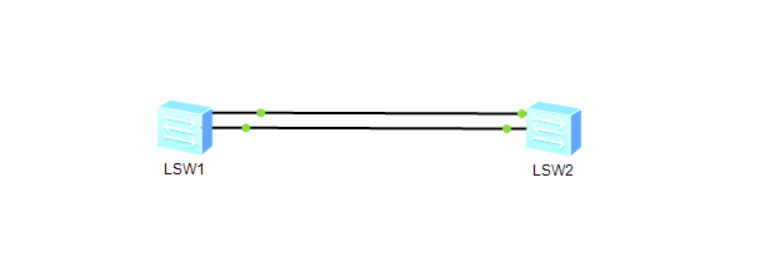
\includegraphics[width=\textwidth]{images/scheme.png}
        \caption{Схема роутеров}
    \end{figure}

    \begin{figure}[H]
        \centering
        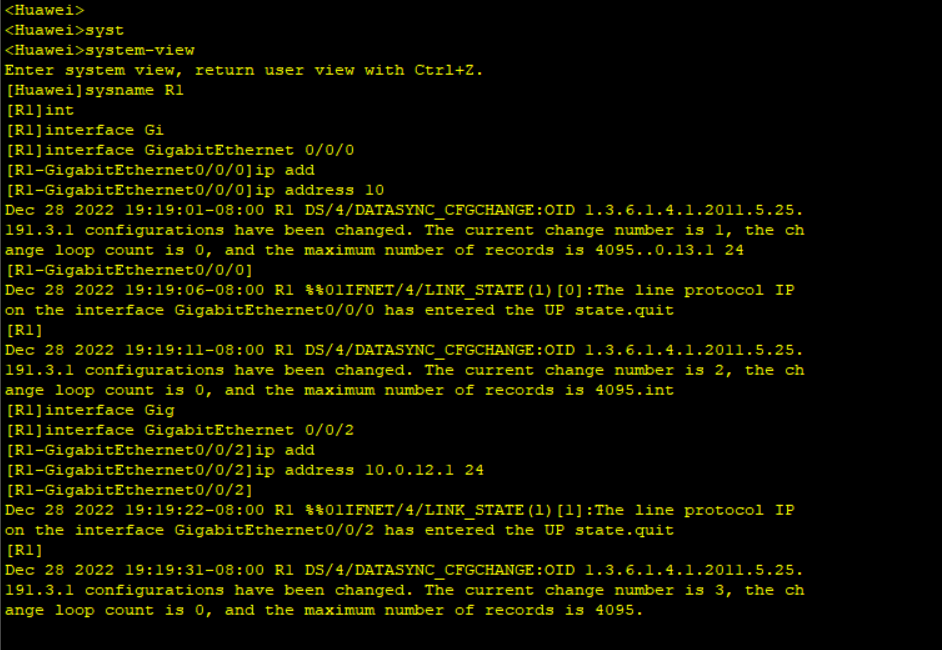
\includegraphics[width=\textwidth]{images/ip_r1.png}
        \caption{Установка IP-адреса на роутер R1}
    \end{figure}

    \begin{figure}[H]
        \centering
        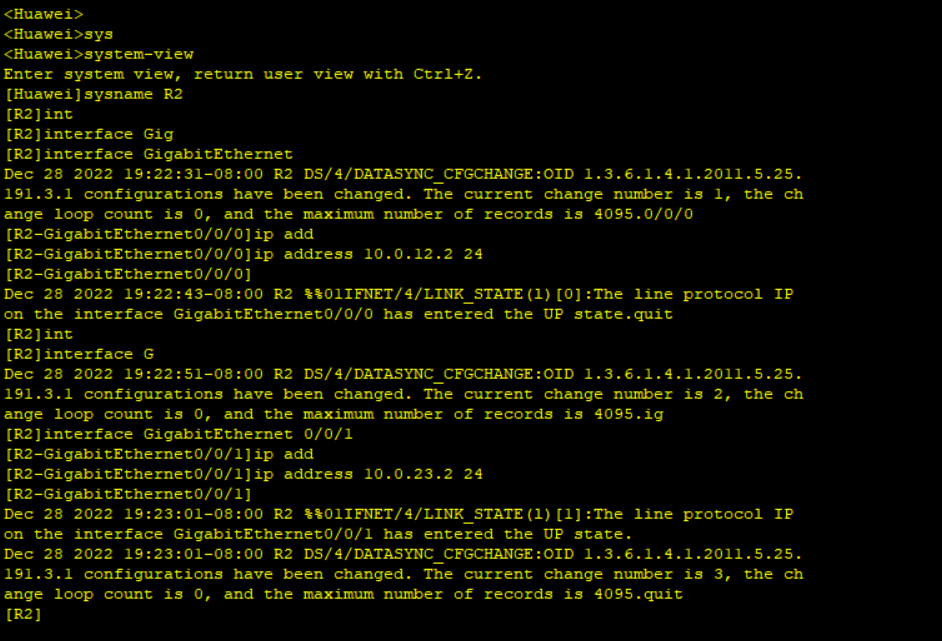
\includegraphics[width=\textwidth]{images/ip_r2.png}
        \caption{Установка IP-адреса на роутер R2}
    \end{figure}

    \begin{figure}[H]
        \centering
        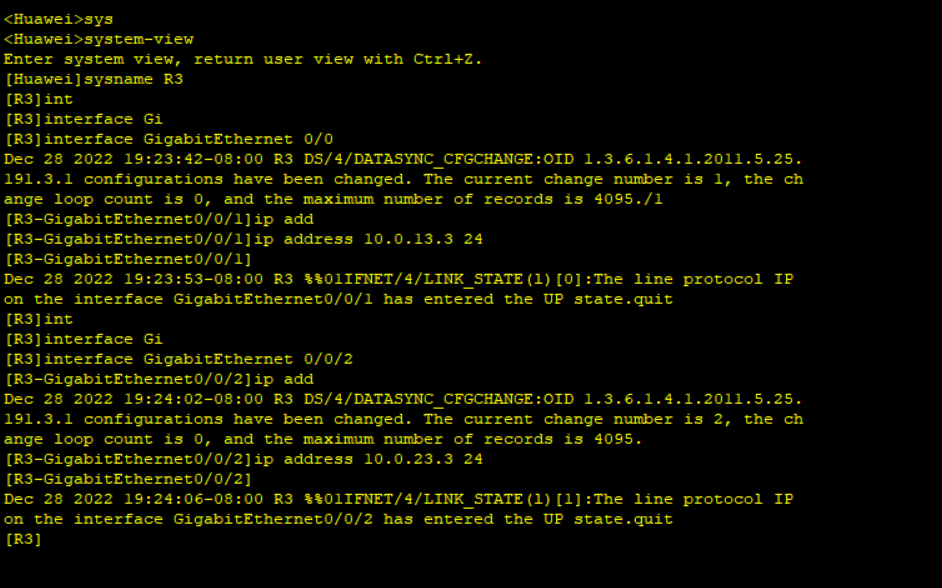
\includegraphics[width=\textwidth]{images/ip_r3.png}
        \caption{Установка IP-адреса на роутер R3}
    \end{figure}

    \begin{figure}[H]
        \centering
        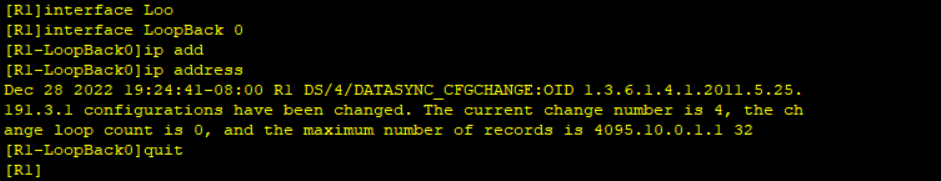
\includegraphics[width=\textwidth]{images/loopback_r1.png}
        \caption{Установка loopback на роутер R1}
    \end{figure}

    \begin{figure}[H]
        \centering
        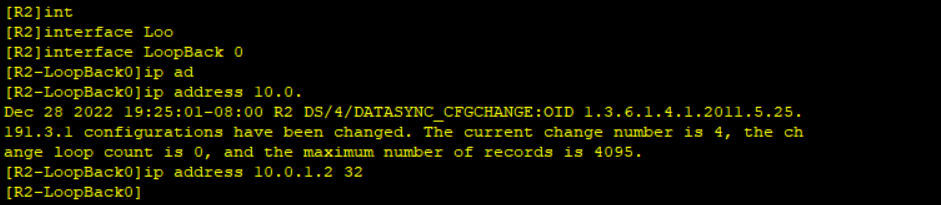
\includegraphics[width=\textwidth]{images/loopback_r2.png}
        \caption{Установка loopback на роутер R2}
    \end{figure}

    \begin{figure}[H]
        \centering
        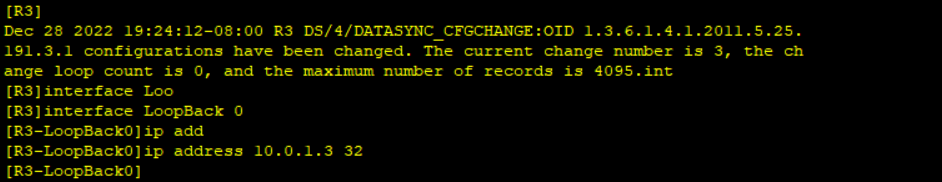
\includegraphics[width=\textwidth]{images/loopback_r3.png}
        \caption{Установка loopback на роутер R3}
    \end{figure}

    \begin{figure}[H]
        \centering
        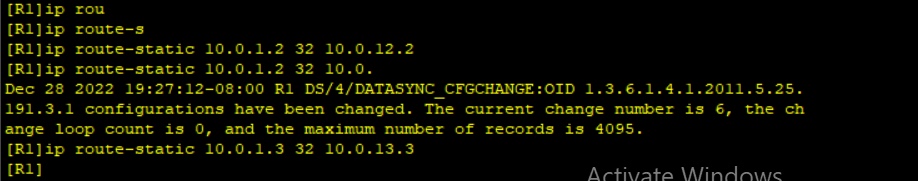
\includegraphics[width=\textwidth]{images/static_ip_r1.png}
        \caption{Установка статического IP-адреса на роутер R1}
    \end{figure}

    \begin{figure}[H]
        \centering
        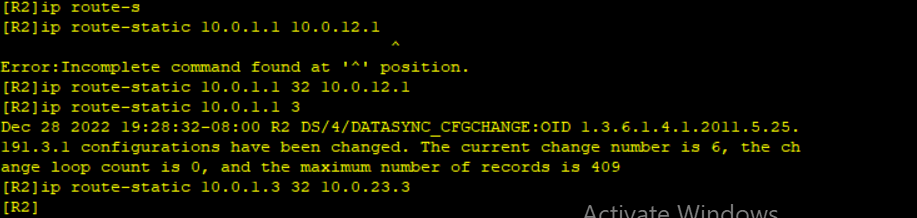
\includegraphics[width=\textwidth]{images/static_ip_r2.png}
        \caption{Установка статического IP-адреса на роутер R2}
    \end{figure}

    \begin{figure}[H]
        \centering
        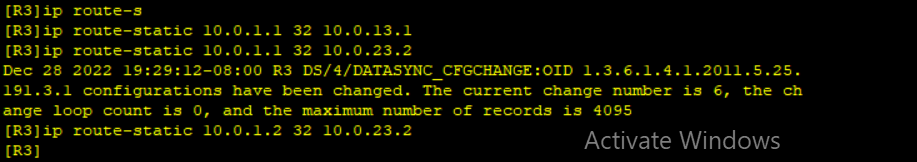
\includegraphics[width=\textwidth]{images/static_ip_r3.png}
        \caption{Установка статического IP-адреса на роутер R3}
    \end{figure}

    \begin{figure}[H]
        \centering
        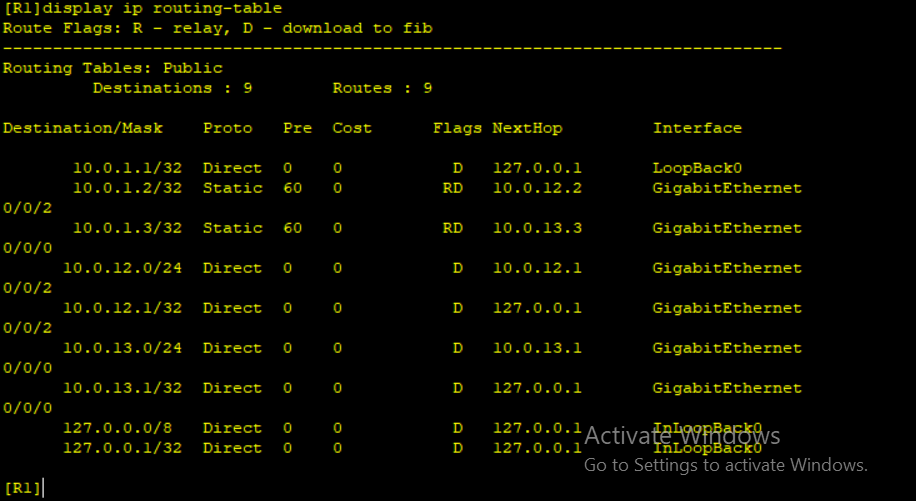
\includegraphics[width=\textwidth]{images/table_r1.png}
        \caption{Таблица IP-адресов на роутере R1}
    \end{figure}

    \begin{figure}[H]
        \centering
        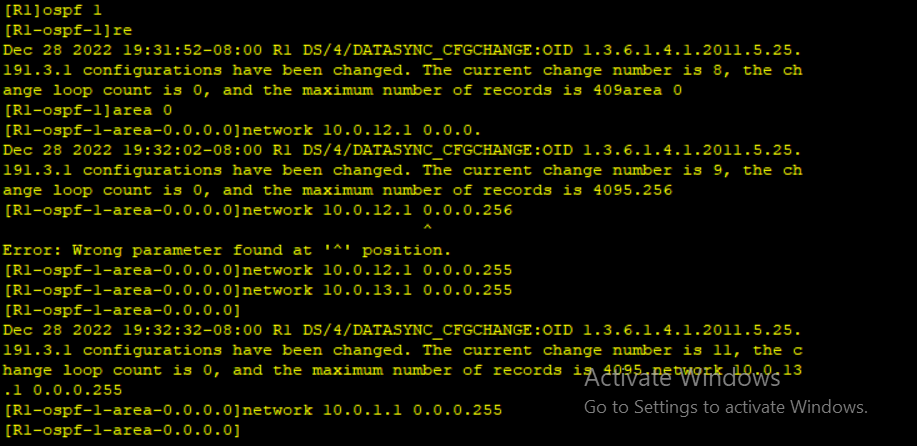
\includegraphics[width=\textwidth]{images/ospf_r1.png}
        \caption{Установка OSPF на роутер R1}
    \end{figure}

    \begin{figure}[H]
        \centering
        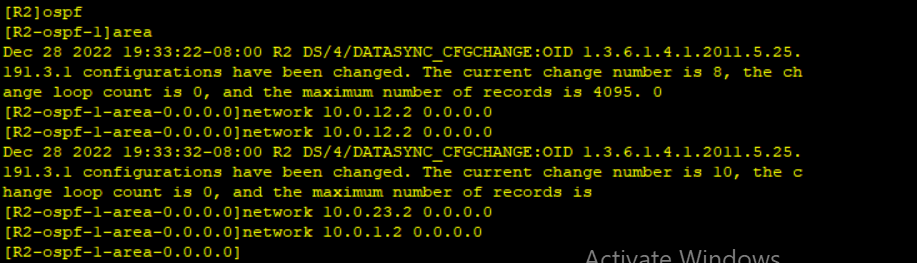
\includegraphics[width=\textwidth]{images/ospf_r2.png}
        \caption{Установка OSPF на роутер R2}
    \end{figure}

    \begin{figure}[H]
        \centering
        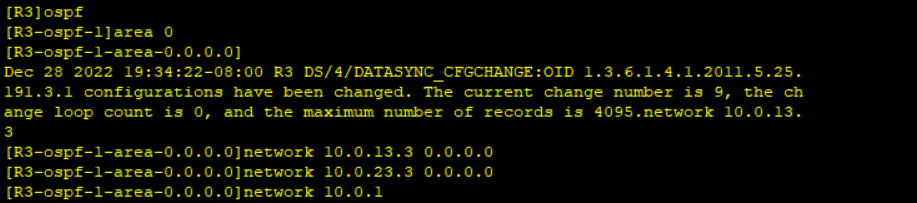
\includegraphics[width=\textwidth]{images/ospf_r3.png}
        \caption{Установка OSPF на роутер R3}
    \end{figure}

    \begin{figure}[H]
        \centering
        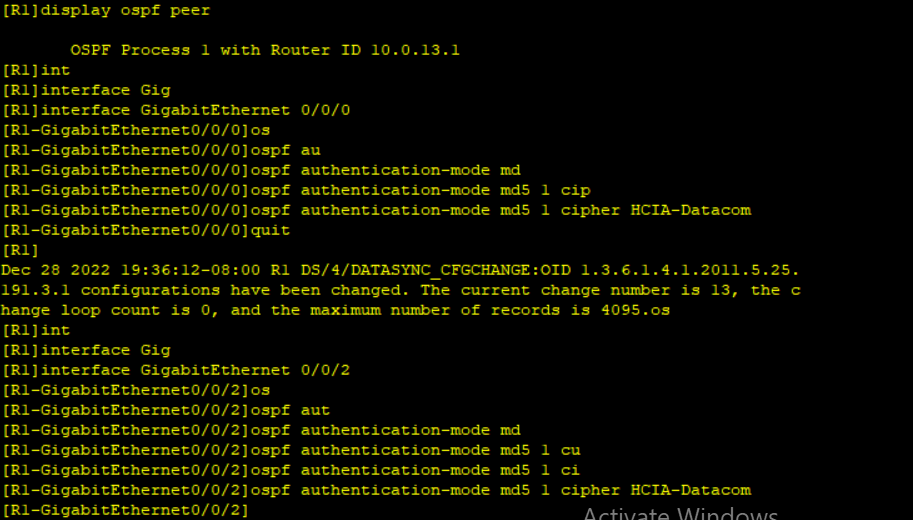
\includegraphics[width=\textwidth]{images/ospf_auth_r1.png}
        \caption{Установка аутентификации OSPF}
    \end{figure}

    \section*{Вопросы}

    \textbf{Какой маршрут будет использоваться на шаге 6 маршрутизатором R2 для возврата пакетов ICMP на маршрутизатор R1?} - через 10.0.13.3 и 10.0.23.2, так как минимальная стоимость.
\end{document}
